\chapter{Tema 6: Support Vector Machines}

\section{Clasificación en 2 clases con Funciones Discriminantes Lineales}

Si usamos dos clases, es muy útil etiquetarlas como -1 y 1 y usar
un único vector de pesos $\theta = \theta_1 - \theta_2$.
De esta forma clasificamos de la siguiente forma:

\begin{itemize}
    \item Clase 1 o +1: $\phi_1(x) \geq \phi_2(x) \Rightarrow \theta_1^t x \geq \theta_2^t x \Rightarrow \theta^t x \geq 0$
    \item Clase 2 o -1: $\phi_1(x) < \phi_2(x) \Rightarrow \theta_1^t x < \theta_2^t x \Rightarrow \theta^t x < 0$
\end{itemize}

Clasificador, $f_{\theta}(x) : \mathbb{R}^n \rightarrow \{-1, 1\}$

\begin{equation*}
    f_{\theta}(x) =
    \begin{cases}
        1 & \text{si } \theta^t x \geq 0 \\
        -1 & \text{si } \theta^t x < 0
    \end{cases}
\end{equation*}

Se define la función discriminante lineal (FDL) como

\begin{equation*}
    \phi: \mathbb{R}^d \rightarrow \mathbb{R} \text{ tal que } 
    \phi(x; \Theta) = \theta^t x + \theta_0 = 
    \sum_{i=1}^{d} \theta_i x_i + \theta_0
\end{equation*}

Donde $\Theta = (\theta, \theta_0)$ : $\theta \in \mathbb{R}^d$ es el 
vector de pesos y $\theta_0 \in \mathbb{R}$ se denomina umbral.
El número de parámetros de $\Theta$ es $D = d+1$.

En forma compacta:

\begin{equation*}
    c_n \cdot (\theta^t x_n + \theta_0) \geq 0 \quad 1 \leq n \leq N
\end{equation*}

Donde $c_n \in \{-1, 1\}$ es la clase de la observación $x_n$.

Frontera de decisión: $F = {x: \theta^t x = 0}$

\textbf{Propiedad:} La distancia de un punto $x$ a la frontera de decisión
($r_x$) es proporcional al valor absoluto de $\theta^t x$:
$r_x \propto |\theta^t x$|

\section{Propiedades de las Funciones Discriminantes Lineales}

\begin{enumerate}
    \item Una FDL, $\phi(x; \Theta)$, define un hiperplano de separación
    $H = {x: \theta^t x + \theta_0 = 0}$.
    \item $H$ divide $\mathbb{R}^d$ en dos semiespacios: $H^+ = {x: \theta^t x + \theta_0 > 0}, c = +1$ y $H^- = {x: \theta^t x + \theta_0 < 0}, c = -1$.
    \item Dado un $\gamma \in \mathbb{R^+}$, entonces $\gamma \cdot \phi(x; \Theta)$ representa el mismo hiperplano $H$.
    \item El vector de pesos $\theta$ es ortogonal a $H$ y su vector unitario es $\frac{\theta}{||\theta||}$.
    \item La distancia de cualquier $x_s$ a $H$ es:
    \begin{align*}
        x_s &= r_{x_s} \frac{\theta}{\|\theta\|} + x_o, \\
        \theta^t x_s &= r_{x_s} \frac{\theta^t \theta}{\|\theta\|} + \theta^t x_o, \\
        \theta^t x_s + \theta_0 &= r_{x_s} \frac{\|\theta\| \|\theta\|}{\|\theta\|} + \underbrace{\theta^t x_o + \theta_0}_{(x_o \in H) \implies 0}, \\
        r_{x_s} &= \frac{\left| \phi(x_s; \Theta) \right|}{\|\theta\|} = \frac{\left| \theta^t x_s + \theta_0 \right|}{\|\theta\|}.
    \end{align*}
    Donde $x_o$ es un punto de $H$.

    \begin{figure}[H]
        \centering
        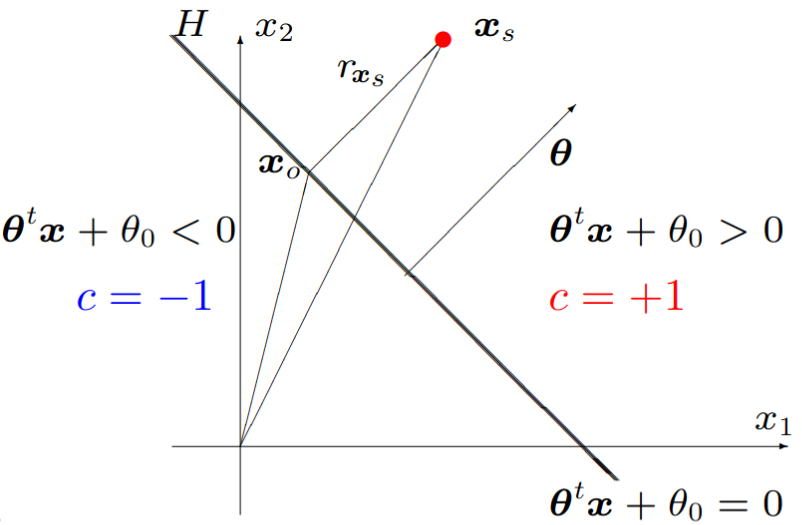
\includegraphics[width=0.5\textwidth]{images/fdl_hiperplano.png}
        \caption{Distancia de un punto a la frontera de decisión.}
    \end{figure}
\end{enumerate}

\section{Hiperplano y márgen de un Hiperplano separador}

\begin{itemize}
    \item Para un conjunto de muestras linealmente separables
    existen infinitos hiperplanos separadores.
    \item El margen $\tau$ de un hiperplano $H$ es la mínima distancia
    entre $H$ y la muestra más cercana a cualquiera de sus clases.
    \begin{equation*}
        \tau = \min_{n} \left| \frac{\theta^t x_n + \theta_0}{\|\theta\|} \right|
    \end{equation*}
    \item Un hiperplano $H$ es óptimo si maximiza el margen $\tau$.
\end{itemize}

\begin{figure}[H]
    \centering
    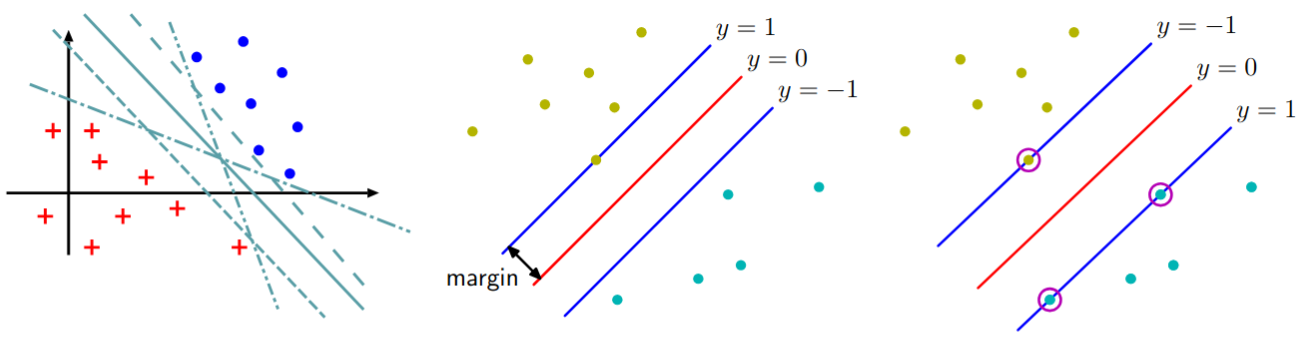
\includegraphics[width=0.8\textwidth]{images/fdl_hiperplano_optimo.png}
    \caption{Hiperplano cualquiera vs Hiperplano óptimo.}
\end{figure}

La distancia de caulquier punto $x_n$ a $H$ será siempre mayor
que el margen $\tau$.

Las muestras de la frontera que delimita el margen (a ambos
lados de $H$) se denominan \textbf{vectores soporte}. Cumplen que:

\begin{equation*}
    \frac{|\phi(x_i; \Theta)|}{\|\theta\|} = \tau \quad \forall x_i \in \mathcal{V}
\end{equation*}

siendo $\mathcal{V}$ el conjunto de todos los vectores soporte.

\subsection{Propiedades de los clasificadores de orden máximo}

Voy a saltarme algunas partes para igualar la clase de hoy

\section{Clase 22 nov. Máquinas de soporte y núcleos}

\subsection{Calcular vector de pesos } $\theta^*$

\subsubsection{Márgenes duros}

$$ \theta^* = \sum_{n=1}^{N} c_n x_n $$

$$ \theta_0^* = c_m - \theta^{*t} x_m , \quad \alpha_m > 0$$

$$ \theta_0^* = c_m - \sum_{n\in \mathcal{V}} c_n \alpha_n  \mathcal{K}(x_n, x_m), \quad \alpha_m > 0$$

\subsection{Márgenes blandos}

$$ \theta^* = \sum_{n=1}^{N} c_n \alpha_n x_n $$

\begin{exercisebox}{Ejercicio 1 GitHub}
    Dado el siguiente conjunto de datos y un Kernel polinómico definido como 

$$ K(x, y) = (\langle x, y \rangle + 1)^2 $$
$$ \langle x, y \rangle = x^t \cdot y = x_1 y_1 + x_2 y_2 $$


Y las muestras:

$( x_1 = [1, 1], c_1 = +1)$

$( x_2 = [0, 0], c_2 = +1)$

$( x_3 = [0, 1], c_3 = -1)$

$( x_4 = [1, 0], c_4 = -1)$

Calcula la matriz Kernel para dichas muestras y resuelve el problema
de clasificación con márgenes duros.

\end{exercisebox}

Tenemmos que ir calculano uno a uno los elementos de la matriz Kernel
aplicando la función Kernel a cada par de muestras.

\begin{itemize}
    % Fila 1
    \item $K(x_1, x_1) = (x_1^t \cdot x_1 + 1)^2 = (2 + 1)^2 = 9$
    \item $K(x_1, x_2) = (x_1^t \cdot x_2 + 1)^2 = (0 + 1)^2 = 1$
    \item $K(x_1, x_3) = (x_1^t \cdot x_3 + 1)^2 = (1 + 1)^2 = 4$
    \item $K(x_1, x_4) = (x_1^t \cdot x_4 + 1)^2 = (1 + 1)^2 = 4$
    % Fila 2
    % La matriz es simétrica, por lo que no es necesario calcular
    % todos los elementos
    \item $K(x_2, x_2) = (x_2^t \cdot x_2 + 1)^2 = (0 + 1)^2 = 1$
    \item $K(x_2, x_3) = (x_2^t \cdot x_3 + 1)^2 = (0 + 1)^2 = 1$
    \item $K(x_2, x_4) = (x_2^t \cdot x_4 + 1)^2 = (0 + 1)^2 = 1$
    % Fila 3
    \item $K(x_3, x_3) = (x_3^t \cdot x_3 + 1)^2 = (1 + 1)^2 = 4$
    \item $K(x_3, x_4) = (x_3^t \cdot x_4 + 1)^2 = (0 + 1)^2 = 1$
    % Fila 4
    \item $K(x_4, x_4) = (x_4^t \cdot x_4 + 1)^2 = (1 + 1)^2 = 4$
\end{itemize}

La matriz Kernel resultante es:

\begin{equation*}
    K =
    \begin{bmatrix}

    9 & 1 & 4 & 4 \\

    1 & 1 & 1 & 1 \\

    4 & 1 & 4 & 1 \\

    4 & 1 & 1 & 4
    \end{bmatrix}
\end{equation*}

Resolvemos el problema de clasificación con márgenes duros (no hay C)

\begin{lstlisting}[language=Python]
from scipy.optimize import minimize
import numpy as np

# Datos y etiquetas
x = np.array([[1, 1], [0, 0], [0, 1], [1, 0]])
labels = np.array([1, 1, -1, -1])
n_samples = len(labels)

# Definición del kernel polinómico
def polynomial_kernel(x, y):
    return (np.dot(x, y) + 1) ** 2



# Construcción de la matriz kernel
kernel_matrix = np.zeros((4, 4))
for i in range(4):
    for j in range(4):
        kernel_matrix[i, j] = polynomial_kernel(x[i], x[j])


# Definir la función objetivo para la optimización dual de SVM
def objective(alphas):
    return 0.5 * np.sum([alphas[i] * alphas[j] * labels[i] * labels[j] * kernel_matrix[i, j] for i in range(n_samples) for j in range(n_samples)]) - np.sum(alphas)

# Restricción: \sum \alpha_i y_i = 0
def constraint_eq(alphas):
    return np.dot(alphas, labels)

# Restricción: \alpha_i >= 0
bounds = [(0, None) for _ in range(n_samples)]

# Punto inicial para la optimización
initial_alphas = np.zeros(n_samples)

# Resolver el problema de optimización
result = minimize(
    fun=objective,
    x0=initial_alphas,
    bounds=bounds,
    constraints={'type': 'eq', 'fun': constraint_eq},
    method='SLSQP'
)

# Extraer los valores de \alpha
optimal_alphas = result.x

print(optimal_alphas)
\end{lstlisting}

Clasificar las muestras de entrenamiento

\begin{equation*}
    f(x_i) = \sum_{n=1}^{N} c_n \alpha_n K(x_n, x_i) + b
\end{equation*}

El sesgo (bias $b$) se puede calcular como:

\begin{equation*}
    b = c_n - \sum_{m\in \mathcal{V}} c_m \alpha_m K(x_n, x_m)
\end{equation*}

\textbf{Calculamos el sesgo}

Por ejemplo, para la muestra $x_1, c_1 = +1$:

\begin{align*}
    b & = \sum_{m = 1}^{4} c_m \alpha_m K(x_m, x_1) \\
    & = +1-(2*9 + 1*(10/3) - 4*(8/3) - 4*(8/3)) \\
    & = 1- (54/3 + 10/3 - 32/3 -32/3) \\
    & = 1-0=1
\end{align*}